\documentclass[11pt]{beamer}
\usepackage{booktabs,siunitx}
\usepackage[compat=1.1.0]{tikz-feynman}
\usepackage[default]{opensans}
\usetheme{Madrid}
\usefonttheme{default}
\useinnertheme{circles}
\sisetup{detect-all}
\setbeamertemplate{navigation symbols}{} % Uncomment this line to remove the navigation symbols from the bottom of all slides

\title[Charged Lepton Flavour Violation]{Charged Lepton Flavour Violation: \\ An Introduction} % The short title in the optional parameter appears at the bottom of every slide, the full title in the main parameter is only on the title page

% \subtitle{Optional Subtitle} % Presentation subtitle, remove this command if a subtitle isn't required

\author[Miles Kidson]{Miles Kidson} % Presenter name(s), the optional parameter can contain a shortened version to appear on the bottom of every slide, while the main parameter will appear on the title slide

\institute[UCT]{University of Cape Town \\ \smallskip \textit{kdsmil001@myuct.ac.za}} % Your institution, the optional parameter can be used for the institution shorthand and will appear on the bottom of every slide after author names, while the required parameter is used on the title slide and can include your email address or additional information on separate lines

\date[November 2022]{November 2022} % Presentation date or conference/meeting name, the optional parameter can contain a shortened version to appear on the bottom of every slide, while the required parameter value is output to the title slide

% \useoutertheme[subsection=false]{miniframes}

\begin{document}

\frame[plain]{\titlepage}

\begin{frame}
    \frametitle{Standard Model conserved quantities}
    \begin{columns}[c]
        \begin{column}{0.6\textwidth}
            There are a few quantities that are strictly conserved in SM processes:
            \bigskip
            \begin{itemize}
                \item Electric \& colour charge
                \item Baryon number $B$
                \item Lepton number $L$
            \end{itemize}
            \bigskip
            If neutrinos were massless, individual lepton flavour numbers $L_e$, $L_\mu$, and $L_\tau$ would be conserved. With massive neutrinos, only $L$ is conserved.

            (Provided neutrinos are Dirac fermions and not Majorana fermions)

        \end{column}
        \begin{column}{0.4\textwidth}
            \begin{figure}[h]
                \begin{center}
                    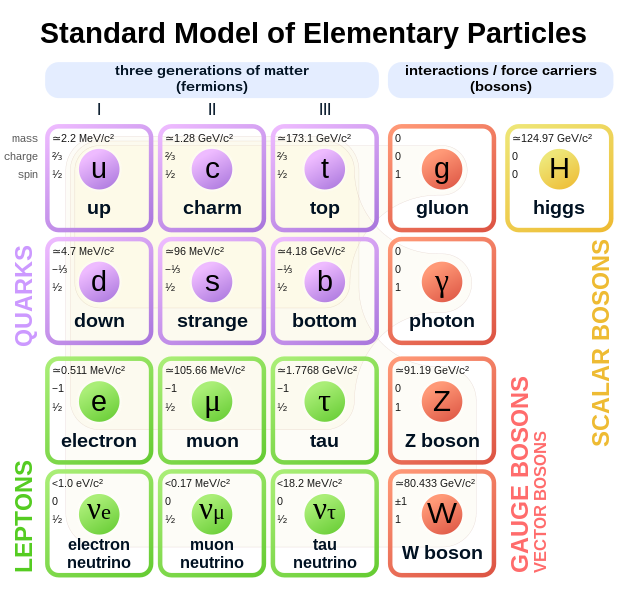
\includegraphics[width=\textwidth]{SM.png}
                \end{center}
            \end{figure}
            
        \end{column}
        
    \end{columns}

    

\end{frame}

\begin{frame}
    \frametitle{Charged Lepton Flavour Violation (CLFV)}
    \begin{columns}[c]
        \begin{column}{0.6\textwidth}
            \begin{itemize}
                \item Example processes would be $\mu \rightarrow e\gamma$, $\mu\rightarrow e\,e\,e$, and $\tau \rightarrow \mu,e + X$
                \item We already see lepton flavour being violated in neutrino oscillation
                \item Best estimates of $\mu \rightarrow e\gamma$ rates by the same mechanism are $<10^{-54}$, which are not realistically measurable
                \item Thus observing these processes implies new physics is at play!
            \end{itemize}
        \end{column}

        \begin{column}{0.4\textwidth}
            \begin{tikzpicture}
                \begin{feynman}
                    \vertex (a);
                    \vertex [right=1cm of a] (b);
                    \vertex [right=1cm of b] (c);
                    \vertex [right=1cm of c] (d);
                    \vertex [right=1cm of d] (e);
                    \vertex [above right=1cm of d] (f);

                    \diagram {
                        (a) -- [fermion, edge label'=$\mu$] (b) -- [fermion, edge label'=$\nu$] (c) -- [fermion, edge label'=$e$] (d) -- [fermion, edge label'=$e$] (e);
                        (b) -- [boson, half left, edge label=$W$] (c);
                        (d) -- [photon, edge label=$\gamma$] (f);
                    };

                \end{feynman}
            \end{tikzpicture}
        \end{column}
    \end{columns}
\end{frame}

\begin{frame}
    \frametitle{Experimental bounds on process rates}
    The best limits on 

    

\end{frame}

\begin{frame}
    \frametitle{MEG detector?}

    

\end{frame}

\begin{frame}
    \frametitle{Best theories for explaining it}

    

\end{frame}

\begin{frame}
    \frametitle{Conclusion}

    

\end{frame}



\end{document}